%; whizzy chapter
% -initex iniptex -latex platex -format platex -bibtex jbibtex -fmt fmt
% 以上 whizzytex を使用する場合の設定。

%     Tokyo Debian Meeting resources
%     Copyright (C) 2006 Junichi Uekawa

%     This program is free software; you can redistribute it and/or modify
%     it under the terms of the GNU General Public License as published by
%     the Free Software Foundation; either version 2 of the License, or
%     (at your option) any later version.

%     This program is distributed in the hope that it will be useful,
%     but WITHOUT ANY WARRANTY; without even the implied warranty of
%     MERCHANTABILITY or FITNESS FOR A PARTICULAR PURPOSE.  See the
%     GNU General Public License for more details.

%     You should have received a copy of the GNU General Public License
%     along with this program; if not, write to the Free Software
%     Foundation, Inc., 51 Franklin St, Fifth Floor, Boston, MA  02110-1301 USA

%   Pdf作成手順
% dvipdfmx debianmeetingresume200606.dvi
%  preview (shell-command (concat "xpdf " (replace-regexp-in-string "tex$" "pdf"(buffer-file-name)) "&"))
% 画像ファイルを処理するためにはebbを利用してboundingboxを作成。
%(shell-command "cd image200606; ebb *.png")

%%ここからヘッダ開始。

\documentclass[mingoth,a4paper]{jsarticle}
\usepackage[dvipdfmx]{graphicx}
\usepackage{fancybox}
\usepackage{longtable}
\usepackage{ascmac}	% 囲み (screen,itembox)
\usepackage{fancyvrb}   % 囲み Verbatim のために必要
\usepackage[dvipdfmx]{hyperref}
\usepackage{url}
\usepackage[dvipdfmx]{color}

%http://www.naney.org/diki/dk/hyperref.html
%日本語EUC系環境の時
\AtBeginDvi{\special{pdf:tounicode EUC-UCS2}}
%シフトJIS系環境の時
%\AtBeginDvi{\special{pdf:tounicode 90ms-RKSJ-UCS2}}

%% spacing の設定をする。外枠を減らす。
\setlength\headheight{0mm}
\setlength\topmargin{-20mm}
\setlength\headsep{0mm}
\setlength\topskip{3mm}
\setlength\maxdepth{4pt}
\setlength\columnsep{6mm}
\setlength\textheight{252mm}
\setlength\topmargin{-5mm}
\setlength\textwidth{170mm}
\setlength\oddsidemargin{-5mm}
\setlength\evensidemargin{-5mm}

% commandline環境を定義。画面入出力についてはcommandline環境
% で表記する
\newenvironment{commandline}%
{\VerbatimEnvironment
  \begin{Sbox}\begin{minipage}{15cm}\begin{fontsize}{7.3}{7.3} \begin{BVerbatim}}%
{\end{BVerbatim}\end{fontsize}\end{minipage}\end{Sbox}
  \setlength{\fboxsep}{8pt}\fbox{\TheSbox}}


%%% start of santaku
\makeatletter
\newwrite\tf@jqz
\immediate\openout\tf@jqz\jobname.jqz\relax
\makeatother
\newcounter{santakucounter}
\newcommand{\santaku}[5]{%
\addtocounter{santakucounter}{1}

\addtocontents{jqz}{\arabic{santakucounter}. #5\\}
\begin{minipage}{1\hsize}
問題\arabic{santakucounter}. 
#1\\
□ A #2\\
□ B #3\\
□ C #4
\end{minipage}
\hspace{1cm}
\\

}
%%% end of santaku

\newcommand{\emptyspace}{(\underline{\hspace{1cm}})}

\newcommand{\subsubsubsection}[1]{%
\vspace{1zw}{\bf #1}\\}


% sectionをセンタリングする
\makeatletter
  \renewcommand{\section}{\@startsection{section}{1}{\z@}%
    {\Cvs \@plus.5\Cdp \@minus.2\Cdp}% 前アキ
    {.5\Cvs \@plus.3\Cdp}% 後アキ
    {\normalfont\Huge\headfont\raggedright\centering}} % style
\makeatother

% section の代わりの環境
\newcommand{\dancersection}[2]{%
\newpage
東京エリアDebian勉強会 2006
\hrule
\vspace{0.5mm}
\hrule
%\hfill{}
\includegraphics[width=3cm]{image200502/openlogo-nd.eps}\\
%\hfill{}
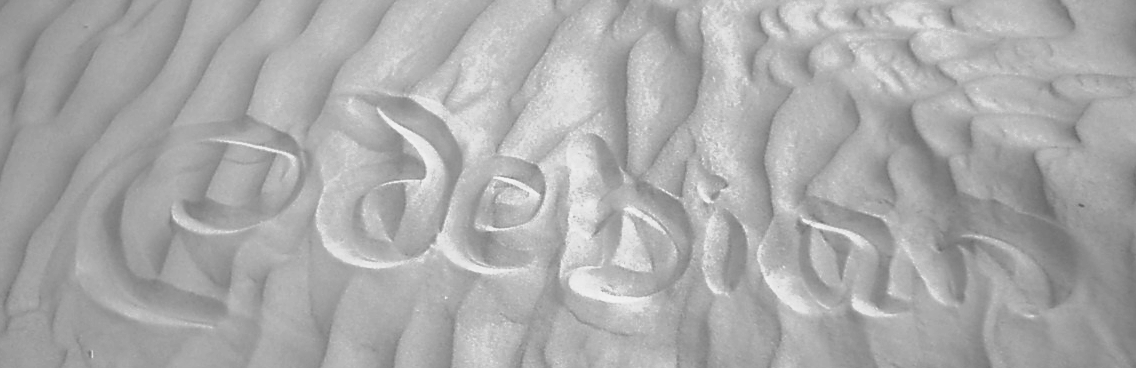
\includegraphics[width=16cm]{image2006-natsu/guruguru-sand-light.png}\\
\vspace{-5cm}
\begin{center}
\section{#1}
\end{center}
\hfill{}\colorbox{white}{#2}\hspace{3cm}\space\\
\vspace{1cm}
\hrule
\vspace{0.5mm}
\hrule
\vspace{1cm}
}

% for dancerj
\newcommand{\fgref}[1]{図\ref{#1}}
\newcommand{\tbref}[1]{表\ref{#1}}


\begin{document}

\begin{titlepage}

% 毎月変更する部分, 本文の末尾も修正することをわすれずに
\title{
 第19回 東京エリア Debian 勉強会\\事前資料}
\date{2006年8月19日}
\author{Debian勉強会会場係 上川 純一\thanks{Debian Project Official Developer}} 
\maketitle
\thispagestyle{empty}
\end{titlepage}

\newpage
\tableofcontents

\dancersection{Introduction To Debian 勉強会}{上川 純一}

今月のDebian勉強会へようこそ。
これからDebianのあやしい世界に入るという方も、すでにどっぷりとつかってい
るという方も、月に一回Debianについて語りませんか?

目的として下記の二つを考えています。

\begin{itemize}
 \item メールではよみとれない、もしくはよみとってられないような情報を情
       報共有する場をつくる
 \item まとまっていないDebianを利用する際の情報をまとめて、ある程度の塊と
       して出してみる
\end{itemize}

また、東京にはLinuxの勉強会はたくさんありますので、Debianに限定した勉強
会にします。Linuxの基本的な利用方法などが知りたい方は、他でがんばってくださ
い。
Debianの勉強会ということで究極的には参加者全員がDebian Packageを
がりがりと作りながらスーパーハッカーになれるような姿を妄想しています。

Debianをこれからどうするという能動的な展開への土台としての空間を提供し、
情報の共有をしたい、というのが目的です。
次回は違うこと言ってるかもしれませんが、御容赦を。

\subsection{講師紹介}

\begin{itemize}
 \item{岩松 信洋} スーパーエッチハッカーです。
 \item{山下さん} 誕生日だそうです。
 \item{野首さん} 今日はパッケージを切ってくれるはずです。
 \item{やまねさん} Debian JP のウェブを改革してくれるそうです。
 \item{上川 純一} 宴会の幹事です。
\end{itemize}

\subsection{事前課題紹介}

今回の事前課題は
「Debian 誕生日に思うこと」、「ysjjさんへの誕生日のメッセージ」もしくは「最近感銘を受けたパッケージ」
というタイトルで200-800文字程度の文章を書いてください。
というものでした。
その課題に対して下記の内容を提出いただきました。

\subsubsection{Debian 誕生日に思うこと 山下 純司さん}

忘れもしないCマガジン1995年10月号特別付録CD-ROMに収録されていた
Linux/TOWNSから始まったLinux生活。本誌に掲載されていたLinux解説記事の
著者が鵜飼さんだったことはDebianに繋がる見えない道標だったのでしょうか。

13年の歴史の中で様々の障害に取り掛かり乗り越えてきたのだと思います。
ソフトウェア特許は難しいながら長年の課題としてあり続けてきたものですが、
私にとって予想外だったのはFDLとの衝突でしょうか。GPLv3も今年中にはっきり
とした形を見せてくる予定だったと思います。

これからもオープンソースライセンスに関してDebianの主導的振舞に
期待しています。

\subsubsection{Debian 誕生日に思うこと 前田 耕平さん}

13周年ですか、13年前はまだDOSとWindowsしか知らなかったです。
Debianは使いはじめて2年強、Linux自体もまだ5年そこそこの新参者なので恐縮ですが、
今後ますます発展してほしいです。まずは自分の周りの人間を引き込むところから始めます。

\subsubsection{最近感銘を受けたパッケージ たかやさん}

私が、最近感銘を受けたパッケージは、現在Debianのオフィシャルパッケージではないが、
howm(一人お手軽Wikiもどき)だ。ソースファイルを見てみたら、
GPLだと書かれていてユーザーも多いみたいなので、
将来的にはDebianのオフィシャルパッケージになるのではないかと思う。
大学に入るまでは、PDAであるVisorEdgeを使って、予定やちょっとしたメモを取ってきたが、
Linuxを本格的に使うようになってから、コマンドが多く適当にディレクトリーを使って、
雑文を保存していた。しかし、最近検索機能などもつけたいし、
予定やtodoとしての機能も使いたいので何かEmacs上で良いソフトがないか調べていたら、
howmを知った。howmは、リンク機能、そして検索機能などもあり、
メモを書くにはかなり便利なソフトだと思われる。

\subsubsection{Debian 誕生日に思うこと キタハラさん}

    「Debian 誕生日」って具体的には何時だろう?
・・・という事で、Google 様に聞いてみてみると、
「Debian 5 回目の誕生日!」という1998年08月13日の
Debian ニュースの記事が見つかった。  と言う事は
1993年08月16日が誕生日って事ですね。

    13 歳というと、人間で言えば小学校卒業して中学
生になった頃でしょうか?  人間ならばこの頃には、相
手がアホでも相手に合わせて会話が出来るようになるの
で、Debian も私のようなアホにも愛想良く簡単に使え
るようになって頂ければ嬉しいなぁ〜、と思います。

    なにはともあれ、13 年目、めでたい事であります。

\subsubsection{最近感銘を受けたパッケージ 平川 佳樹}

自分は元々redhat9からLinuxを使い始めた人間なのですが
apt・dpkgやupdate-alternatives・kernel-package等のシステム管理のパッケージが気に入っています。
独自の使い方やルール等の感覚をつかむまでよくわかりませんでしたが
これらのパッケージの存在のお陰でシステムの基盤をお好みに構築するのは
他ディストリビューションと比べても結構スムーズに出来る気がします。
システムの依存関係もめちゃくちゃになりにくいのも助かっています。

\subsubsection{Debian 誕生日に思うこと えとーさん}

なんだかしらないが時間ばっかり過ぎている自分と比べて徐々に
成長しているような気がする「Debian」はすごいなぁと思う。

最初期から活動してきた人とかはどんどん減って
新しい人がどんどん入っているのかなぁ(日本除く)と思う。

13周年というと、徐々に枯れたプロジェクトになって行くのだろうか?

13歳と言うともう中学生、つまり「チュウボウ」なので、反抗期みたいな
尖ったプロジェクトになって行くのだろうか?

今年(?)はetchをリリースするようだけど今後の安定的なリリースのために
大きな一歩になる年になるのだろうか。

今年も楽しみなプロジェクトです。
今年こそもう少しなんかできるといいなぁ。

\subsubsection{Debian 誕生日に思うこと 南谷さん}

あれはたしか小学校高学年、あるいは中学校に入学した直後だったと思
う。
ちょうど算数・数学でxを用いた方程式を学習する時期であった。
導入として以下のような問題の解き方を考えさせられた。
同じような問題を解かされた方も少なくないと思う。

龍三郎さんは現在47歳です。
香織さんは21歳です。
龍三郎さんの年齢が香織さんの年齢のちょうど倍になるのは何年後でしょ
う。

答えは以下の方程式を解くことで求められる。
47+x=2(21+x)
x=5

さてDebian は13歳の誕生日だそうだが、Debianの年齢とみなさんの年齢を用いてこの
方程式を組み立て、解いてみていただきたい。

今、日本のDebian 開発者、OSS開発者に特に求められているのはx<0の人材で
はないだろうか。
x<0 の方々にはどうどうと胸を張って大いにあばれていただきたい。

かくいう私はx=3です。
失礼しました。

\subsubsection{岩松 信洋}

数年前までは Debian? Linux? ハァ? と言う感じでしたが、今ではどっぷり使って Debian を
開発する側に回ってしまいました。今ではもっと先に Debian と戯れていたらなぁと思っています。
13 終年 にならないよう、今後もがんばっていけたらなぁと思います。

\subsubsection{上川}

Debian も、もう13周年です。
よくわからないですが、老舗です。
また、Debian は常に変化しています。
毎年違う姿を見せてくれているように思います。
波瀾万丈、また愉しきかな。

今後ともよろしくお願いします。


\subsubsection{今日のコメント}

{\LARGE 
(\hspace{5cm})さん: (\hspace{5cm})の話をした。\\
(\hspace{6cm})の点がよかった。\\
(\hspace{6cm})すればもっとよくなるだろう。\\
}

{\LARGE 
(\hspace{5cm})さん: (\hspace{5cm})の話をした。\\
(\hspace{6cm})の点がよかった。\\
(\hspace{6cm})すればもっとよくなるだろう。\\
}

{\LARGE 
(\hspace{5cm})さん: (\hspace{5cm})の話をした。\\
(\hspace{6cm})の点がよかった。\\
(\hspace{6cm})すればもっとよくなるだろう。\\
}

{\LARGE 
(\hspace{5cm})さん: (\hspace{5cm})の話をした。\\
(\hspace{6cm})の点がよかった。\\
(\hspace{6cm})すればもっとよくなるだろう。\\
}

{\LARGE 
(\hspace{5cm})さん: (\hspace{5cm})の話をした。\\
(\hspace{6cm})の点がよかった。\\
(\hspace{6cm})すればもっとよくなるだろう。\\
}

%%% trivia quiz
\dancersection{Debian Weekly News trivia quiz}{上川 純一}

ところで、Debian Weekly News (DWN)は読んでいますか?
Debian 界隈でおきていることについて書いているDebian Weekly News.
毎回読んでいるといろいろと分かって来ますが、一人で読んでいても、解説が少
ないので、
意味がわからないところもあるかも知れません。みんなでDWNを読んでみましょう。

漫然と読むだけではおもしろくないので、DWNの記事から出題した以下の質問にこたえてみてください。
後で内容は解説します。

\subsection{2006年25号}
\url{http://www.debian.org/News/weekly/2006/25/}
にある6月20日版です。

\santaku
{Isaac Clerencia さんは、スペイン
のサラゴサ市当局が、6 ヶ所ある場所に Debian ベースのシンク
ライアントを設置したと報告しました。その場所とはどこでしょうか}
{ラーメン屋}
{コンビニエンスストア}
{老人ホーム}
{C}

\santaku
{Yaroslav Halchenkoさんが Debian Packge 内のあるファイルが圧縮されていて、読むことが出来ないと気がつきました。
そのファイルとは何でしょうか。}
{Word ファイル}
{PDF ファイル}
{SREC ファイル}
{B}

\subsection{2006年26号}
\url{http://www.debian.org/News/weekly/2006/26/}
にある6月27日版です。

\santaku
{9月にイタリアのある都市でDebian コミュニティカンファレンスがおこなわれます。
そのある都市とはどこでしょう。}
{ベニス}
{デセンツァーノ・デル・ガルーダ}
{カリブ島}
{A}

\santaku
{最近セキュリティチームのメンバーが増えました。それはだれでしょうか。}
{Steve Kemp}
{Hidehazu Koiwa}
{Andreas Barth}
{A}

\subsection{2006年27号}
\url{http://www.debian.org/News/weekly/2006/27/}
にある7月4日版です。
\santaku
{最近また新しいOSにDebianを移植している噂があるらしい。それはどのOSか?}
{Plan9}
{Minix3}
{Mona}
{B}

\santaku
{Paul Wise さんがあたらしいグループを作成しました。それはどのグループか?}
{debian-smoker}
{debian-soccer}
{debian-flash}
{C}

\dancersection{最近のDebian関連のミーティング報告}{上川 純一}

\subsection{東京エリアDebian勉強会18回目報告}
% (query-replace-regexp "<.*>" "")

7月のDebian勉強会は北海道で開催されました。
上川が Debian の紹介、Debian勉強会の紹介、
MacBook に Debian をインストールする方法について説明しました。

今回の参加人数は40人くらいでした。

会場でMacBookをすでに購入しているひとは数人でした。今回の参加によって東
京でのDebian勉強会に参加しようと思った人は5人くらいいました。

\subsection{TLUG}

2006年7月29日、「TLUG」にて Debian を Macbook にインストールする方法に
ついて報告してきました。英語で発表しました。プレゼンテーションを Front
Row コントローラでやったのは好評だったようです。Debianユーザは少数派だっ
たようなので、Debianの普及につながればよいですね。

\dancersection{Debconf in Japan 北海道の検討について}{岩松 信洋}
\label{sec:iwamatsudebconf}

\subsection{はじめに}

	7/14 から 7/17 まで 上川と岩松は札幌に行きました。
	Debconf を 札幌で行うことが可能か、情報収集および打ち合わせをしてきました。
	その報告を行います。

\subsection{札幌 までの道のり	}
札幌に行くための旅路は以下の通りです。

今回は東京から参加したので羽田空港からとなります。

\begin{itemize}
 \item       各都内の駅 $\rightarrow$  浜松町
 \item       浜松町  $\rightarrow$ 東京モノレール 第2空港ビル下車 (約20分) 470円
 \item       羽田空港  $\rightarrow$ 新千歳空港 (約1時間30分)
 \item       新千歳空港  $\rightarrow$ JR札幌駅 (約40分) 1040円
\end{itemize}

海外の方が札幌まで行く場合は

\begin{itemize}
 \item      成田空港到着
 \item       成田空港  $\rightarrow$ 新千歳空港
 \item       新千歳空港   $\rightarrow$ JR 札幌駅
\end{itemize}

     成田空港 - 新千歳空港は1日以下の便があります。

\begin{tabular}[t]{|cc|c|}
\hline
\hline
 & 便名 & 時刻 \\
\hline
      ANA	&	3121 &	10:30→12:05 	  \\
     ANA	&	2155 &	17:55→19:30 	 \\
     日本航空&	3047	&18:40→20:20  \\
\hline
\end{tabular}
 	 
本数が少ないので、海外からの参加者をまとめてピックアップできそうです。

\subsection{産業省さんとの検討内容}
通産省の方と札幌で Debconf を開催したときにどのような問題があるか、どのような場所を提供できるか
等、お話しました。担当者はまるまるさんと言って、北海道での OSS に関する活動をサポートされてい
る方です、

\subsubsection{市立大学}
\begin{itemize}
	\item WebSite : \url{http://www.scu.ac.jp}
	\item 森の中にある。
	\item 交通は不便。
	\item 泊まるところもない。テント張る?
\end{itemize}

\subsubsection{コンベンションセンターはどうか}

\begin{itemize}
	\item Website : \url{http://www.sora-scc.jp/}
	\item 場所が遠い。
	\item 泊まるところが近くにない。
	\item ネットワークがなく、別途引く必要あり。
	\item 時間の制限がある可能性がある。	
\end{itemize}


\subsubsection{学術工芸会館}
\begin{itemize}
	\item 大聖堂がある。オペラ等で使うのでちょっと違う。
	\item ネットワークがない。
\end{itemize}

\subsubsection{時期は?}
\begin{itemize}
	\item 5月はいい季節。
	\item 寒いので汗をかかない。風呂にあまり入らないハッカーとその回りの人にはいい時期。
\end{itemize}
	
\subsubsection{組織の問題}

○○実行委員会とか。
ビザの発行手続きの問題があるので必要。
\footnote{ビザの発行については外務省のページに詳しい 
\url{http://www.mofa.go.jp/mofaj/toko/visa/annai/visa_5.html}}

\subsection{北海道大学さんとの検討内容}

Debconf を北海道大学さんで行う場合に北海道大学さんとして、どのように協力していた
だけるか、というお話をしました。

\subsubsection{セッション/BOF等}
	学術交流会館
	情報教育館(日本PostgreSQLユーザ会北海道支部が使っているらしい。)
	
\subsubsection{ハックラボ}
	北海道大学情報科学研究科棟(OSC Hokakido 開催場所)
	

\subsubsection{検討事項}

\begin{itemize}
 \item  宿泊施設に関して: \\
	場所は北海道大学の講義室を借りることが可能。
	しかし、北海道大学周辺には大規模な宿泊施設がなく、ハックラボやセッション	
	への移動が困難である。北海道大学を中心で行う場合は、この問題を解決する必要がある。

 \item  時間の制限: \\
	各部屋を利用する場合、使用する時間が設けられているため、21時ぐらいに部屋を
	出ないといけない。これは開催側からハックできる場所が提供できないということ
	なので、問題である。できればハックできる時間を多くとらせてあげたいので、長
	時間、できれは24時間体制で提供できるようにする必要がある。

 \item  電源の問題: \\
	古い建物では電源に関してあまり考えられてないため、300人近くが同時にPCを
	立ち上げたりすると、電源容量の問題が発生する。
	北海道大学は場所によっては問題なく使用できるところがあるが、場所が離れている
	ため、移動が困難。ハックラボとセッション、BOFができる部屋はできるだけ近くで
	行えるようにしたい。

 \item  食事: \\
	食堂のプリペイドカードが使える。
	開催時は食堂のメニューにベジタリアン用メニューを作ってもらう。
\end{itemize}


\subsection{その他}


\begin{tabular}{ll}
   会社の研修施設: &
	企業が利用している 研修施設を利用するのはどうか?\\
  交通: &
	成田から北海道までの交通費が高い。往復で5万円する。\\
\end{tabular}

\subsection{下見をしたところ}

	札幌ゲストハウス(札幌天神山国際ハウス): 
	丘の上にある。地下鉄東西線の澄川駅の近く。
	30人ぐらいしか泊まれない。

\dancersection{module-assistant}{上川}
\label{sec:modass}

Debian 用にカーネルモジュールパッケージを作成する方法について解説します。

\subsection{従来の方法、kernel-package}

従来は、kernel-package にて実装されていた方法を利用することが多かったで
す。最近は、その簡便さから流行はmodule-assistantに移行しはじめているよう
です。

\subsection{module-assistantの利用}

\texttt{module-assistant} はパッケージのインストール、ソースの展開、
ビルド、インストールまでの一連の作業を自動化してくれるツールです。

まず、カーネルソースの場所を教えます。通常、現在実行中のカーネルに対して
のソースのディレクトリは\texttt{/lib/modules/\$(uname -r)/build}のシンボ
リックリンクをたどることで取得できます。そのため、何も指定しないで下記の
コマンドをうつと設定できます。

\begin{commandline}
 # m-a prepare
\end{commandline}

一度カーネルソース、もしくはカーネルヘッダパッケージを適切にインストール・
設定したあとはパッケージ名を指定してあげれば、そのパッケージからモジュー
ルを作成し、インストールするところまで実施してくれます。

\begin{commandline}
 # m-a a-i \textit{package}
\end{commandline}

このコマンドを入力すると、\textit{package}-source パッケージをインストー
ルし、/usr/src/\textit{package}.tar.bz2を展開、モジュールパッケージをビ
ルドして、パッケージをインストールしてくれます。

出力例を見てみましょう。

\begin{commandline}
# m-a --text-mode a-i linux-uvc
.
1 パッケージについての情報を更新しました
Getting source for kernel version: 2.6.18-rc2dancer-gb4e54de8-dirty
/lib/modules/2.6.18-rc2dancer-gb4e54de8-dirty/source のカーネルヘッダを利用できます
apt-get install build-essential
パッケージリストを読み込んでいます... 完了
依存関係ツリーを作成しています... 完了
build-essential はすでに最新バージョンです。
アップグレード: 0 個、新規インストール: 0 個、削除: 0 個、保留: 122 個。

完了!
download
パッケージリストを読み込んでいます... 完了
依存関係ツリーを作成しています... 完了
以下のパッケージが新たにインストールされます:
  linux-uvc-source
アップグレード: 0 個、新規インストール: 1 個、削除: 0 個、保留: 122 個。
32.7kB 中 0B のアーカイブを取得する必要があります。
展開後に追加で 73.7kB のディスク容量が消費されます。
パッケージフィールドを読み込んでいます... 完了
パッケージ状態を読み込んでいます... 完了
バグレポートを取得しています... 完了
未選択パッケージ linux-uvc-source を選択しています。
(データベースを読み込んでいます ... 現在 131883 個のファイルとディレクトリがインストールされています。)
(.../linux-uvc-source_0.1.0-2_amd64.deb から) linux-uvc-source を展開しています...
linux-uvc-source (0.1.0-2) を設定しています ...
linux-uvc-source についての情報を更新中

1 パッケージについての情報を更新しました
unpack
Extracting the package tarball, /usr/src/linux-uvc.tar.bz2, please wait...
"/usr/share/modass/packages/default.sh" build
 KVERS=2.6.18-rc2dancer-gb4e54de8-dirty 
 KSRC=/lib/modules/2.6.18-rc2dancer-gb4e54de8-dirty/source KDREV=GIT.2006.07.25.15.08 kdist_image
dh_testdir
dh_testroot
dh_clean
/usr/bin/make -C /usr/src/modules/linux-uvc clean \
        KERNELPATH=/lib/modules/2.6.18-rc2dancer-gb4e54de8-dirty/source 
KERNELRELEASE=2.6.18-rc2dancer-gb4e54de8-dirty
 KERNELCONF=/lib/modules/2.6.18-rc2dancer-gb4e54de8-dirty/source/.config 

[中略]

dh_builddeb --destdir=/home/dancer/shared/git
tar: -: file name read contains nul character
dpkg-deb:
 /home/dancer/shared/git/linux-uvc-modules-2.6.18-rc2dancer-gb4e54de8-dirty_0.1.0-2+GIT.2006.07.25.15.08_amd64.deb 
にパッケージ `linux-uvc-modules-2.6.18-rc2dancer-gb4e54de8-dirty' を構築しています。
make[1]: ディレクトリ `/usr/src/modules/linux-uvc' から出ます
/usr/bin/make  -f debian/rules kdist_clean
make[1]: ディレクトリ `/usr/src/modules/linux-uvc' に入ります
dh_testdir
dh_testroot
dh_clean
/usr/bin/make -C /usr/src/modules/linux-uvc clean \
        KERNELPATH=/lib/modules/2.6.18-rc2dancer-gb4e54de8-dirty/source
 KERNELRELEASE=2.6.18-rc2dancer-gb4e54de8-dirty
 KERNELCONF=/lib/modules/2.6.18-rc2dancer-gb4e54de8-dirty/source/.config 
make[2]: ディレクトリ `/usr/src/modules/linux-uvc' に入ります
rm -f *.o *.ko .*.cmd .*.flags *.mod.c Modules.symvers
rm -rf .tmp_versions
make[2]: ディレクトリ `/usr/src/modules/linux-uvc' から出ます
make[1]: ディレクトリ `/usr/src/modules/linux-uvc' から出ます
dpkg -Ei
 /home/dancer/shared/git/linux-uvc-modules-2.6.18-rc2dancer-gb4e54de8-dirty_0.1.0-2+GIT.2006.07.25.15.08_amd64.deb 
未選択パッケージ linux-uvc-modules-2.6.18-rc2dancer-gb4e54de8-dirty を選択しています。
(データベースを読み込んでいます ... 現在 131888 個のファイルとディレクトリがインストールされています。)
(.../linux-uvc-modules-2.6.18-rc2dancer-gb4e54de8-dirty_0.1.0-2+GIT.2006.07.25.15.08_amd64.deb
 から) linux-uvc-modules-2.6.18-rc2dancer-gb4e54de8-dirty を展開していま
 す... 
linux-uvc-modules-2.6.18-rc2dancer-gb4e54de8-dirty (0.1.0-2+GIT.2006.07.25.15.08) を設定しています ...

\end{commandline}

\subsection{パッケージの作成方法}

まず、カーネルモジュールのソースを提供するためのパッケージを作成します。
今回の例では、\texttt{tt-source}パッケージです。\texttt{module-assistant}から処理
できるように、\texttt{パッケージ名-source }という命名規則に従ってくださ
い。\texttt{tt-source}パッケージはモジュールのソースを
\texttt{/usr/src/package.tar.bz2}をインストールします。
\texttt{/usr/src/package.tar.bz2} の中身自体は、またDebianソースパッケー
ジの形態になっており、\texttt{module-assistant} が処理してカーネルモジュー
ルパッケージを生成できるようになっています。

\texttt{module-assistant}用のソースの中に debian/*.modules.in というファイル名で
おいてあると、その中にある \texttt{\_KVERS\_} と書いている部分がカーネル
のバージョン番号に置換されます。
登場するファイルの代表的なものを簡単に説明します。

\begin{itemize}
 \item \texttt{rules}
 \item \texttt{control.modules.in}: モジュールパッケージのコントロールファイルで
       す。
 \item \texttt{postinst.modules.in}: インストールされたときに実行されます。depmod
       などを実行します。
\end{itemize}

\subsubsection{dh-make を利用した例}

\texttt{dh\_make}を利用して作成してみましょう。ドライバの名前は仮に \texttt{tt} とします。

\begin{commandline}
$ dh_make

Type of package: single binary, multiple binary, library, kernel module or cdbs?
 [s/m/l/k/b] k

Maintainer name : Junichi Uekawa
Email-Address   : dancer@debian.org
Date            : Sat, 29 Jul 2006 13:13:32 +0900
Package Name    : tt
Version         : 1
License         : blank
Type of Package : Kernel Module
Hit <enter> to confirm:
Skipping creating ../tt_1.orig.tar.gz because it already exists
Done. Please edit the files in the debian/ subdirectory now. You should also
check that the tt Makefiles install into $DESTDIR and not in / .
\end{commandline}

作成されるソースパッケージのディレクトリ構造は下記のようになっています。

\begin{itemize}
 \item driver/: ドライバのソース
 \item ./: 通常のソース
 \item debian/: debianの通常のソースパッケージに必要なもろもろのファイル
\end{itemize}

パッケージを作成してdebc で確認してみます。tt-source というパッケージが
できています。/usr/src/tt.tar.bz2 というファイルが作成されています。この
中身を作成するのがメインの仕事になります。

\begin{commandline}
 tt-source_1-1_all.deb
 ---------------------
 新形式 debian パッケージ、バージョン 2.0。
 サイズ 5608 バイト: コントロールアーカイブ = 576 バイト。
     466 バイト,    13 行      control
     199 バイト,     3 行      md5sums
 Package: tt-source
 Version: 1-1
 Section: unknown
 Priority: optional
 Architecture: all
 Depends: module-assistant, debhelper (>> 4.0.0), make, bzip2
 Installed-Size: 12
 Maintainer: Junichi Uekawa <dancer@debian.org>
 Source: tt
 Description: Source for the tt driver.
  This package provides the source code for the tt kernel modules.
  The tt package is also required in order to make use of these
  modules. Kernel source or headers are required to compile these modules.
 drwxr-xr-x root/root         0 2006-07-29 13:27 ./
 drwxr-xr-x root/root         0 2006-07-29 13:27 ./usr/
 drwxr-xr-x root/root         0 2006-07-29 13:27 ./usr/share/
 drwxr-xr-x root/root         0 2006-07-29 13:27 ./usr/share/doc/
 drwxr-xr-x root/root         0 2006-07-29 13:27 ./usr/share/doc/tt-source/
 -rw-r--r-- root/root       188 2006-07-29 13:13 ./usr/share/doc/tt-source/changelog.Debian.gz
 -rw-r--r-- root/root       627 2006-07-29 13:13 ./usr/share/doc/tt-source/copyright
 drwxr-xr-x root/root         0 2006-07-29 13:27 ./usr/src/
 -rw-r--r-- root/root      3832 2006-07-29 13:27 ./usr/src/tt.tar.bz2

 tt_1-1_i386.deb
 ---------------
 新形式 debian パッケージ、バージョン 2.0。
 サイズ 1928 バイト: コントロールアーカイブ = 452 バイト。
     243 バイト,     8 行      control
     197 バイト,     3 行      md5sums
 Package: tt
 Version: 1-1
 Section: unknown
 Priority: optional
 Architecture: i386
 Installed-Size: 12
 Maintainer: Junichi Uekawa <dancer@debian.org>
 Description: <insert up to 60 chars description> <insert long description, indented with spaces>
 drwxr-xr-x root/root         0 2006-07-29 13:27 ./
 drwxr-xr-x root/root         0 2006-07-29 13:27 ./usr/
 drwxr-xr-x root/root         0 2006-07-29 13:27 ./usr/share/
 drwxr-xr-x root/root         0 2006-07-29 13:27 ./usr/share/doc/
 drwxr-xr-x root/root         0 2006-07-29 13:27 ./usr/share/doc/tt/
 -rw-r--r-- root/root       188 2006-07-29 13:13 ./usr/share/doc/tt/changelog.Debian.gz
 -rw-r--r-- root/root       627 2006-07-29 13:13 ./usr/share/doc/tt/copyright
 -rw-r--r-- root/root       926 2006-07-29 13:13 ./usr/share/doc/tt/README.Debian
 drwxr-xr-x root/root         0 2006-07-29 13:27 ./usr/sbin/
 drwxr-xr-x root/root         0 2006-07-29 13:27 ./usr/bin/

\end{commandline}

\texttt{tt.tar.bz2} の中身をみてみましょう。

\begin{commandline}
$ tar tfj tt-source/usr/src/tt.tar.bz2 
 modules/
 modules/tt/
 modules/tt/Makefile
 modules/tt/debian/
 modules/tt/debian/compat
 modules/tt/debian/copyright
 modules/tt/debian/changelog
 modules/tt/debian/rules
 modules/tt/debian/tt-modules-_KVERS_.postinst.modules.in.ex
 modules/tt/debian/control.modules.in
\end{commandline}

通常の Debian のソースパッケージの形になっています。これらは、
\texttt{make-kpkg} か、\texttt{module-assistant}から利用されることを想定
しています。\texttt{debian/rules} はそのままコピーしてきたものを利用して
います。\texttt{binary-modules}という特別なターゲットが準備してあり、モ
ジュールをビルドする際に呼び出されます。\texttt{binary-modules} は通常の
カーネルのモジュールのビルドと同じことをします。注意するべきは、Debian 
パッケージを作成するために、実行時に必要なディレクトリ
(\texttt{/lib/modules/}以下) に直接インストールするのではなく、deb パッ
ケージとして配布するためのディレクトリにインストールするという点です。

\begin{commandline}
 cp drivers/slusb.$ko drivers/slamr.$ko debian/$(PKGNAME)/lib/modules/$(KVERS)/misc
\end{commandline}

\texttt{control.modules.in} の中身を見てみます。カーネルのバージョンによっ
て置換される文字列が \texttt{\_KVERS\_} という文字列になっています。
\texttt{control.modules.in} は \texttt{module-assistant} などにより処理
され、各バージョン用の内容に変更されます。同様に、\texttt{\_KVERS\_} を
置換してもらうことを前提として、 \texttt{postinst.modules.in} などを作
成することが可能です。

\begin{commandline}
Source: tt
Section: unknown
Priority: optional
Maintainer: Junichi Uekawa <dancer@debian.org>
Build-Depends: debhelper (>> 4.0.0)
Standards-Version: 3.7.2

Package: tt-modules-_KVERS_
Architecture: any
Provides: tt-modules
Description: tt modules for Linux (kernel _KVERS_).
 This package contains the set of loadable kernel modules for the
 <description>.
 .
 This package contains the compiled kernel modules for _KVERS_
 .
 If you have compiled your own kernel, you will most likely need to build
 your own tt-modules. The tt-source package has been
 provided for use with the Debian's module-assistant or kernel-package
 utilities to produce a version of tt-module for your kernel.
\end{commandline}


\subsubsection{cdbs を利用した例}

madwifi カーネルモジュールなどは \texttt{cdbs} を利用したパッケージ構成になっていま
す。それでは、\texttt{cdbs} を利用した例を見てみましょう。debhelper のみを利用して
いる場合、テンプレート的に毎回同様の内容を記述する部分が多数ありますが、
\texttt{cdbs} を利用することによって、その部分を \texttt{cdbs}に任せ、差異のある部分に集中す
ることができます。

それでは例で見てみましょう。

まず、メインの \texttt{debian/rules} を見てみます。
ここでは、 \texttt{linux-uvc} パッケージを例にとります。

\begin{commandline}
#!/usr/bin/make -f
#mostly copied from madwifi debian/rules

include /usr/share/cdbs/1/rules/debhelper.mk
include /usr/share/cdbs/1/rules/dpatch.mk
include /usr/share/dpatch/dpatch.make

build/linux-uvc-tools::
	-$(MAKE) extract

install/linux-uvc-source::
	# Enforce executable bit on debian/rules, and create directory 
	# structure for modules source
	install -D -m 0755 debian/rules.modules \
		debian/tmp/modules/linux-uvc/debian/rules
	# Prepare the other debian stuff
	for f in *.modules.in control compat copyright changelog README.Debian; do \
		install -m 0644 debian/$$f \
			debian/tmp/modules/linux-uvc/debian/; \
	done
	# Prepare upstream source
	find . -path ./debian/\* -type d -prune -o -printf "%P\n" | \
		egrep -v 'debian|contrib|regression|.svn' | \
		cpio -admp debian/tmp/modules/linux-uvc/
	# clean it
	-$(MAKE) -C debian/tmp/modules/linux-uvc/ clean
	-rm -f debian/tmp/modules/linux-uvc/extract
	# Prepare the debian source tarball
	tar jcf debian/linux-uvc-source/usr/src/linux-uvc.tar.bz2 \
		-C debian/tmp modules

install/linux-uvc-tools::
	install -D -m 0755 extract debian/linux-uvc-tools/usr/sbin/macbook-isight-firmware-loader

clean::
	-rm -f extract
\end{commandline}

\texttt{cdbs}では、各 build ターゲットと install ターゲットを \texttt{build/パッケージ名} 、
\texttt{install/パッケージ名}として定義しているのがわかります。また、dh\_系のコマ
ンドがまったく書かれていません。\texttt{debian/rules -p} を実行すると、それが\texttt{cdbs}
にてどういう風に補完されるのかが確認できます。たとえば、\texttt{linux-uvc-source }
については、おおざっぱに把握すると下記のように展開されることがわかります。

\begin{commandline}
install/linux-uvc-source::
	# Enforce executable bit on debian/rules, and create directory 
	# structure for modules source
	install -D -m 0755 debian/rules.modules \
	debian/tmp/modules/linux-uvc/debian/rules
	# Prepare the other debian stuff
	for f in *.modules.in control compat copyright changelog README.Debian; do \
	install -m 0644 debian/$$f \
	debian/tmp/modules/linux-uvc/debian/; \
	done
	# Prepare upstream source
	find . -path ./debian/\* -type d -prune -o -printf "%P\n" | \
	egrep -v 'debian|contrib|regression|.svn' | \
	cpio -admp debian/tmp/modules/linux-uvc/
	# clean it
	-$(MAKE) -C debian/tmp/modules/linux-uvc/ clean
	-rm -f debian/tmp/modules/linux-uvc/extract
	# Prepare the debian source tarball
	tar jcf debian/linux-uvc-source/usr/src/linux-uvc.tar.bz2 \
	-C debian/tmp modules
	
binary-install/linux-uvc-source::
	dh_installdocs -p$(cdbs_curpkg) $(DEB_INSTALL_DOCS_ALL) $(DEB_INSTALL_DOCS_$(cdbs_curpkg)) 
	dh_installexamples -p$(cdbs_curpkg) $(DEB_INSTALL_EXAMPLES_$(cdbs_curpkg))
	dh_installman -p$(cdbs_curpkg) $(DEB_INSTALL_MANPAGES_$(cdbs_curpkg)) 
	dh_installinfo -p$(cdbs_curpkg) $(DEB_INSTALL_INFO_$(cdbs_curpkg)) 
	dh_installmenu -p$(cdbs_curpkg) $(DEB_DH_INSTALL_MENU_ARGS)
	dh_installcron -p$(cdbs_curpkg) $(DEB_DH_INSTALL_CRON_ARGS)
	dh_installinit -p$(cdbs_curpkg) $(if
 $(DEB_UPDATE_RCD_PARAMS),--update-rcd-params="$(call
 cdbs_strip_quotes,$(DEB_UPDATE_RCD_PARAMS))",$(if
 $(DEB_UPDATE_RCD_PARAMS_$(cdbs_curpkg)),--update-rcd-params="$(call
 cdbs_strip_quotes,$(DEB_UPDATE_RCD_PARAMS_$(cdbs_curpkg)))"))
 $(DEB_DH_INSTALLINIT_ARGS)  
	dh_installdebconf -p$(cdbs_curpkg) $(DEB_DH_INSTALLDEBCONF_ARGS)
	dh_installemacsen -p$(cdbs_curpkg) $(if
 $(DEB_EMACS_PRIORITY),--priority=$(DEB_EMACS_PRIORITY)) $(if
 $(DEB_EMACS_FLAVOR),--flavor=$(DEB_EMACS_FLAVOR))
 $(DEB_DH_INSTALLEMACSEN_ARGS) 
	dh_installcatalogs -p$(cdbs_curpkg) $(DEB_DH_INSTALLCATALOGS_ARGS)
	dh_installpam -p$(cdbs_curpkg) $(DEB_DH_INSTALLPAM_ARGS)
	dh_installlogrotate -p$(cdbs_curpkg) $(DEB_DH_INSTALLLOGROTATE_ARGS)
	dh_installlogcheck -p$(cdbs_curpkg) $(DEB_DH_INSTALLLOGCHECK_ARGS)
	dh_installmime -p$(cdbs_curpkg) $(DEB_DH_INSTALLMIME_ARGS)
	dh_installchangelogs -p$(cdbs_curpkg)
 $(DEB_DH_INSTALLCHANGELOGS_ARGS) $(DEB_INSTALL_CHANGELOGS_ALL)
 $(DEB_INSTALL_CHANGELOGS_$(cdbs_curpkg)) 
	$(if $(wildcard /usr/bin/dh_installudev),dh_installudev -p$(cdbs_curpkg) $(DEB_DH_INSTALLUDEV_ARGS))
	dh_install -p$(cdbs_curpkg) $(if
 $(DEB_DH_INSTALL_SOURCEDIR),--sourcedir=$(DEB_DH_INSTALL_SOURCEDIR))
 $(DEB_DH_INSTALL_ARGS) 
	dh_link -p$(cdbs_curpkg) $(DEB_DH_LINK_ARGS) $(DEB_DH_LINK_$(cdbs_curpkg))
	
\end{commandline}

実行されているおかげで、debhelper 関連のコードを直接記述する必要が無くな
りました。

ただ、\texttt{linux-uvc}はモジュールのビルド用の rules ファイルを分離しています。
\texttt{cdbs} の記述ときれいに分離するための措置です。
\texttt{debian/rules.modules}というものを別途用意しており、それをモジュー
ルのソースの\texttt{debian/rules}として利用しています。\texttt{module-assistant}
自体は \texttt{cdbs} がなくても動作するので、モジュールソースパッケージをインストールする
エンドユーザが追加で \texttt{cdbs} をインストールする必要がないという点も重要かも
しれません。

\begin{commandline}
#!/usr/bin/make -f

PACKAGE := linux-uvc-modules
MA_DIR ?= /usr/share/modass
-include $(MA_DIR)/include/generic.make
-include $(MA_DIR)/include/common-rules.make

.PHONY: kdist_config
kdist_config: prep-deb-files

.PHONY: binary-modules
binary-modules: kdist_config
	dh_testdir
	dh_testroot
	dh_clean -k
	# Build modules
	$(MAKE) -C $(CURDIR) uvcvideo \
	KERNELPATH=$(KSRC) KERNELRELEASE=$(KVERS) KERNELCONF=$(KSRC)/.config 
	# Install modules
	$(MAKE) -C $(CURDIR) install \
	KERNELPATH=$(KSRC) KERNELRELEASE=$(KVERS) KERNELCONF=$(KSRC)/.config \
	INSTALL_MOD_PATH=$(CURDIR)/debian/$(PKGNAME)
 KMODPATH=/lib/modules/$(KVERS)/kernel/drivers/usb/media 
	# remove depmod result
	-rm -f $(CURDIR)/debian/$(PKGNAME)/lib/modules/$(KVERS)/modules.*

	dh_installdocs
	dh_installchangelogs
	dh_compress
	dh_fixperms
	dh_installmodules
	dh_installdeb
	dh_gencontrol -- -v$(VERSION)
	dh_md5sums
	dh_builddeb --destdir=$(DEB_DESTDIR)

.PHONY: kdist_clean
kdist_clean:
	dh_testdir
	dh_testroot
	dh_clean
	$(MAKE) -C $(CURDIR) clean \
	KERNELPATH=$(KSRC) KERNELRELEASE=$(KVERS) KERNELCONF=$(KSRC)/.config 
 
\end{commandline}

\subsection{参考文献}

今回の参考になった資料です。

\begin{itemize}
 \item CDBSのルールを展開して出力する方法\\
       \url{http://syn.theti.ca/articles/2006/07/27/plumbing-the-depths-of-cdbs}
 \item man 8 module-assistant
 \item man dh\_make
 \item テンプレート \url{/usr/share/doc/module-assistant/examples/templates-debian-dir.tar.bz2}
\end{itemize}


\dancersection{コミケ70の報告}{岩松 信洋}

Debian勉強会で作成した資料を本にし、コミックマーケットで販売をしました。
以下に報告します。

\subsection{イベントについて}
\begin{tabular}{|l|l|}
\hline 
イベント名 &

	コミックマーケット 70\\
\hline
 開催日時&

	2006年08月13日\\
\hline
 場所 &

	東京ビックサイト\\
\hline
 出展 & 

	行いませんでした\\ 
\hline
 委託先 &

	美紗緒ネットワーク さん\\
\hline
\end{tabular}	

美紗緒ネットワーク さん
	御協力ありがとうございました。

\subsection{本の内容}

	2006年12回勉強会から2005年17回勉強会の勉強会資料

	2006年12回勉強会から2006年17回勉強会 Debian Weekly News trivia quiz および 答え

\subsection{印刷}
\begin{tabular}{|l|r|}
 
 \hline 印刷所 &
		キンコーズ 市ヶ谷店\\
 \hline 印刷数 &

		80部\\
 \hline 表紙代 &

		608円\\
 \hline 中閉じ代 &

		12000円\\
 \hline コピー代 &

		36000円\\
 \hline 宅急便 &

		1500円\\
 \hline 小計 &

		50108円\\
 \hline 消費税 & 

		2505円\\
 \hline 合計 &
	
		52613円\\
\hline
\end{tabular}



\subsection{販売結果}
\begin{tabular}{|l|r|}
 
\hline 販売金額 &

		800円\\

\hline 販売部数&
 
		79部(1冊はサンプルとして提出。)\\

\hline 売上げ&
 
		63200円( 800円*79部 )\\
\hline
\end{tabular}

\subsection{次回のコミケ}
次回も参加する予定です。回を重ねるたびにページ数が増えているので
次回からは中とじできないようです。オフセットで作ることも考えない
といけません。

\newpage

\vspace*{15cm}
\hrule
\vspace{2mm}

\includegraphics[width=2cm]{image200502/openlogo-nd.eps}
\noindent \Large \bf Debian 勉強会資料\\ \\
\noindent \normalfont 2006年8月19日 \hspace{5mm}  初版第1刷発行\\
\noindent \normalfont 東京エリア Debian 勉強会 (編集・印刷・発行)\\
\hrule

\end{document}
